\chapter{Digital Control and Firmware}
\label{ch:control}

Burst-enable control was developed to regulate the secondary bulk while retaining a fixed carrier. Startup requires precharge before isolated feedback becomes valid; loaded operation requires increased transfer, while load removal requires rapid energy reduction. The controller addresses these conditions using continuous acquisition, voltage feedback, and separate startup, loaded, and no-load states.

The baseline and V2 firmware sources are included in Appendix~\ref{app:full-embedded-source}.

\section{Firmware Development and Versions}
\label{sec:ctrl-firmware-identities}

Control development progressed from manual switching commands through
blocking voltage feedback to continuous ADC acquisition by direct memory
access (DMA). The resulting voltage-control baseline was used for the
main final test series and retained in the integrated V2 port. The later V2
firmware adds calibration and timing controls without changing the bulk-voltage
control law. These additions are described in Section~\ref{sec:ctrl-pwr2-port}.

Table~\ref{tab:ctrl-software-identities} lists the two firmware programs
included with this thesis. The \texttt{PWR} labels are software versions;
V1, V2, and V3 refer to the boards.

\begin{table}[htbp]
\centering
\small
\caption{Firmware versions.}
\label{tab:ctrl-software-identities}
\begin{tabularx}{\textwidth}{@{}L{0.22\textwidth}L{0.19\textwidth}Y@{}}
\toprule
Firmware & Version & Use\\
\midrule
Baseline voltage-control firmware & PWR-1.9.20 & Used in the main V1.0 test series; individual run versions are listed with the results\\
V2 controller firmware & PWR-2.0.4 & Browser calibration, reference-load settings, and adjustable carrier frequency and dead time on V2.\\
\bottomrule
\end{tabularx}
\end{table}
\FloatBarrier

The software history and source-file details are given in
Appendix~\ref{app:firmware}.

\section{Regulating the Secondary Bulk Voltage}
\label{sec:ctrl-objectives}

The enable envelope controls secondary precharge, bulk-voltage regulation, load-removal response, and fault inhibition without changing carrier timing.

The baseline regulates secondary-bulk voltage \(V_{\mathrm{sb}}\) using PA1 feedback; the MPQ4242 USB-C PD stage regulates the output voltage to the selected PD level. Primary-voltage feedback at PA0 supports optional line feed-forward duty limiting. Primary half-bridge current at PA2 provides load classification and optional current protection, rather than direct USB-C output-current feedback.

On the original prototype, average energy transfer is adjusted through burst-enable duty \(d_{\mathrm{EN}}\) at PA10. Carrier outputs PA8/PA9 remain fixed at \SI{1}{\mega\hertz}.

\section{ADC Sampling and Burst Timing}
\label{sec:ctrl-architecture}

The Arduino STM32 framework was used with direct peripheral configuration. Center-aligned TIM1 generates the carrier commands at PA8/PA9: \SI{1}{\mega\hertz} with a nominal \SI{40}{\nano\second} dead interval at both transitions. TIM3 schedules burst enable at PA10. Before non-static enable transitions, bounded polling attempts to align the edge with a TIM1 update; timeout can occur without an observed update. Static \SI{100}{\percent} command holds PA10 high without repeated gaps. A low enable inhibits further switching but does not discharge the power-circuit capacitors.

ADC1 sequentially samples primary voltage at PA0, secondary-bulk voltage at PA1, and half-bridge current at PA2 into a circular DMA buffer. The scan is free-running without synchronization to the carrier, and DMA acquisition continues while the foreground loop runs. Each control pass converts and filters the latest samples, evaluates state and faults, and sends a duty request to the enable scheduler. A hardware UART carries commands and status.

\begin{figure}[htbp]
\centering
\begingroup
\definecolor{ctrlnavy}{HTML}{153448}
\definecolor{ctrlteal}{HTML}{007C83}
\definecolor{ctrlred}{HTML}{990000}
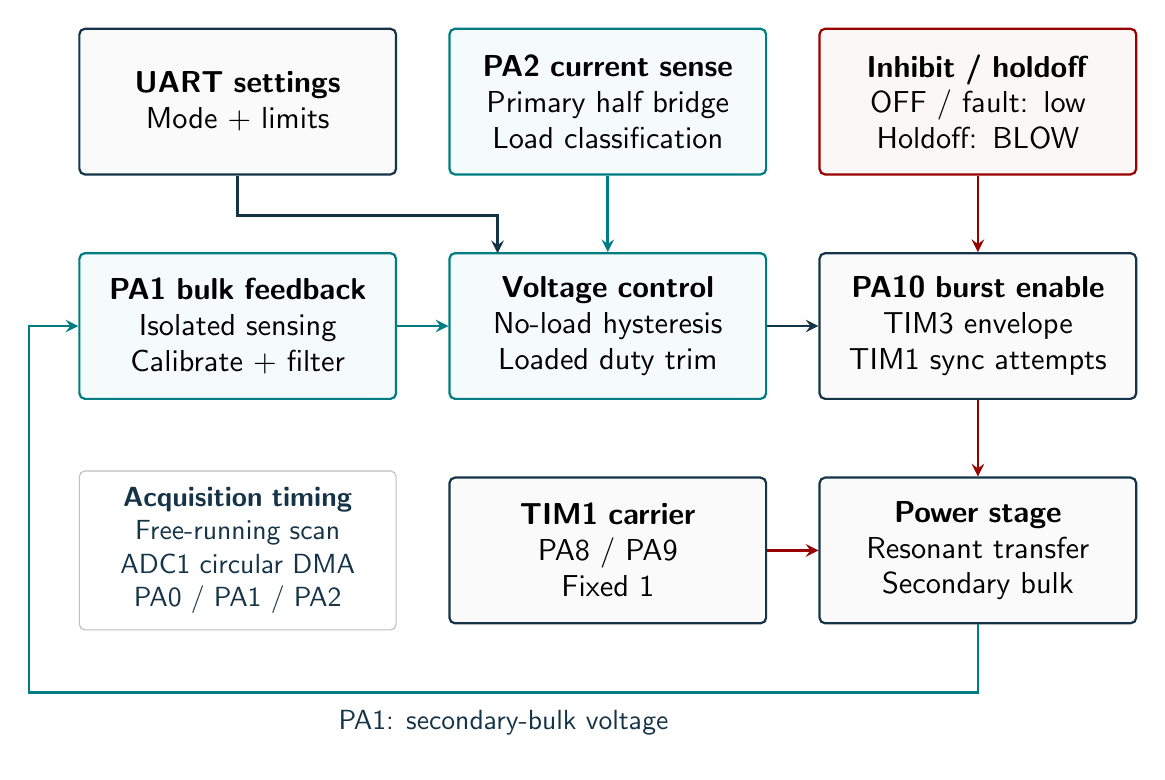
\begin{tikzpicture}[
font=\sffamily\fontsize{11}{13}\selectfont,
every node/.style={align=center,inner sep=6pt,
    execute at begin node={\hyphenpenalty=10000\exhyphenpenalty=10000}},
block/.style={draw=ctrlnavy,fill=black!2,rounded corners=2pt,
    line width=0.8pt,text width=3.6cm,minimum height=1.85cm},
ctrl/.style={block,draw=ctrlteal,fill=ctrlteal!4},
protect/.style={block,draw=ctrlred,fill=ctrlred!3},
flow/.style={->,>=stealth,draw=ctrlnavy,line width=1.0pt},
senseflow/.style={flow,draw=ctrlteal},
command/.style={flow,draw=ctrlred},
annotation/.style={font=\sffamily\fontsize{10}{12}\selectfont,text=ctrlnavy}]
\node[ctrl] (sense) at (0,0)
    {\textbf{PA1 bulk feedback}\\Isolated sensing\\Calibrate + filter};
\node[ctrl] (control) at (4.7,0)
    {\textbf{Voltage control}\\No-load hysteresis\\Loaded duty trim};
\node[block] (en) at (9.4,0)
    {\textbf{PA10 burst enable}\\TIM3 envelope\\TIM1 sync attempts};
\node[block] (plant) at (9.4,-2.85)
    {\textbf{Power stage}\\Resonant transfer\\Secondary bulk};
\node[block] (uart) at (0,2.85)
    {\textbf{UART settings}\\Mode + limits};
\node[ctrl] (load) at (4.7,2.85)
    {\textbf{PA2 current sense}\\Primary half bridge\\Load classification};
\node[protect] (fault) at (9.4,2.85)
    {\textbf{Inhibit / holdoff}\\OFF / fault: low\\Holdoff: BLOW};
\node[block] (carrier) at (4.7,-2.85)
    {\textbf{TIM1 carrier}\\PA8 / PA9\\Fixed \SI{1}{\mega\hertz}};
\node[annotation,draw=black!25,fill=white,rounded corners=2pt,
    text width=3.6cm,minimum height=1.85cm] at (0,-2.85)
    {\textbf{Acquisition timing}\\Free-running scan\\ADC1 circular DMA\\PA0 / PA1 / PA2};
\draw[senseflow] (sense) -- (control);
\draw[flow] (control) -- (en);
\draw[command] (en) -- (plant);
\draw[senseflow] (load) -- (control);
\draw[flow] (uart.south) -- (0,1.4) -- (3.3,1.4) -- (3.3,0.925);
\draw[command] (fault) -- (en);
\draw[command] (carrier) -- (plant);
\draw[senseflow] (plant.south) -- (9.4,-4.65) --
    node[annotation,below,fill=white] {PA1: secondary-bulk voltage}
    (-2.65,-4.65) -- (-2.65,0) -- (sense.west);
\end{tikzpicture}
\endgroup
\caption{Baseline control loop and timing. PA1 provides secondary-bulk voltage feedback; PA2 provides primary-current feedback for load detection. PA10 enables bursts and PA8/PA9 generate the fixed carrier. OFF/fault drives PA10 low; soft holdoff requests \texttt{BLOW}, which is zero by default.}
\label{fig:ctrl-software-architecture}
\end{figure}

\begin{table}[htbp]
\centering
\caption{Timers, ADC, and UART used by the baseline firmware.}
\label{tab:fw-identity-timing-record}
\begin{tabularx}{\textwidth}{@{}p{0.22\textwidth}p{0.27\textwidth}X@{}}
\toprule
Peripheral & MCU pins & Function\\
\midrule
TIM1 & PA8 and PA9 & Fixed carrier and attempts to align enable edges\\
TIM3/GPIO & PA10 & Enable-period scheduling and power-stage inhibition\\
ADC1/DMA1 & PA0, PA1, PA2 & Continuous sampling of the three inputs\\
Hardware UART & PC5 RX, PC4 TX & \SI{115200}{baud} commands, status, and export\\
\bottomrule
\end{tabularx}
\end{table}

Background command parsing is bounded per pass, and settings writes are inhibited while output is enabled to limit control delays. Software counters record observed execution intervals; external timing captures are needed to measure their jitter.

\section{Feedback Conversion and Calibration}
\label{sec:ctrl-feedback}

For a 12-bit ADC count \(N_i\), the input voltage is reconstructed from the configured reference:
\begin{equation}
 V_{\mathrm{ADC},i}=\frac{N_i}{4095}V_{\mathrm{ref}}.
 \label{eq:ctrl-adc-voltage}
\end{equation}
Divider and isolation-amplifier scaling, followed by gain and offset correction, gives the secondary-bulk estimate from PA1:
\begin{equation}
 \widehat V_{\mathrm{sb}}=
 G_{\mathrm{sec}}
 \frac{2V_{\mathrm{clip}}}{V_{\mathrm{AMC,ref}}}
 \left(V_{\mathrm{ADC},1}-\frac{V_{\mathrm{AMC,ref}}}{2}\right)
 \frac{R_{\mathrm{top}}+R_{\mathrm{bottom}}}{R_{\mathrm{bottom}}}
 +V_{\mathrm{off}}.
 \label{eq:ctrl-secondary-calibration}
\end{equation}
The clipping and reference terms describe the configured AMC0330 behavior. \(G_{\mathrm{sec}}\) and \(V_{\mathrm{off}}\) are the gain and offset corrections.

The source defaults are a \SI{3.3}{\volt} ADC/reference setting and a \SI{390}{\kilo\ohm}/\SI{10}{\kilo\ohm} secondary divider. These must match the actual circuit before the voltage thresholds can be relied on. The reference changes between drawings in \cref{sec:hw-sensing} must be checked by measuring the circuit voltage and corresponding ADC-pin voltage.

\begin{table}[htbp]
\centering
\caption{ADC calibration settings in the configuration export.}
\label{tab:fw-calibration-fields}
\begin{tabularx}{\textwidth}{@{}p{0.12\textwidth}p{0.40\textwidth}X@{}}
\toprule
MCU pin & Settings & Purpose\\
\midrule
All & \texttt{VREF} & ADC conversion scale\\
PA0 & \texttt{VPRITOP}, \texttt{VPRIBOT}, \texttt{VPRIGAIN}, \texttt{VPRIOFF} & Primary-voltage conversion\\
PA1 & \texttt{AMCREF}, \texttt{AMCVCLIP}, \texttt{VSECTOP}, \texttt{VSECBOT}, \texttt{VSECGAIN}, \texttt{VSECOFF} & Secondary-bulk voltage conversion\\
PA2 & \texttt{CSRES}, \texttt{CSGAIN}, \texttt{CSOFF}, \texttt{IABS} & Current-signal scaling and zero\\
\bottomrule
\end{tabularx}
\end{table}

Fresh secondary-voltage samples can reduce transfer before the filtered estimate responds. Filtered values reduce noise sensitivity in load classification and duty adjustment, at the cost of delay that must be assessed with the burst pattern.

Calibration and threshold changes can alter the response without changing the firmware version, so the settings must be recorded with each test. External measurements of connector voltage, load current, and AC input power provide the performance calculations and a check on the controller readings.

\section{Control Development}
\label{sec:ctrl-comparison}

Control development addressed manual voltage adjustment, blocking conversion waits, an unsuitable feedback quantity, and excess energy transfer during startup or after load removal (\Cref{tab:ctrl-version-identity}). Each stage changed how the switching bursts responded to the converter and its load.

\begin{table}[htbp]
\centering
\caption{Firmware changes and their functional improvements.}
\label{tab:ctrl-version-identity}
\begin{tabularx}{\textwidth}{@{}L{0.17\textwidth}L{0.37\textwidth}Y@{}}
\toprule
Stage & Change & Improvement\\
\midrule
Open loop & Manual carrier and burst-enable commands & Check switching timing and basic transfer before adding automatic voltage control\\
Blocking feedback & Voltage feedback with blocking ADC reads & Adjust transfer from the sensed voltage instead of relying on manual correction\\
DMA feedback & Continuous ADC DMA and corrected feedback scaling & Remove conversion waits and regulate bulk voltage from PA1 rather than an unsuitable voltage--current product\\
Final baseline & Burst-edge alignment attempts, startup precharge, no-load guard, and loaded duty trim & Limit commanded energy at startup and no load, reduce continued charging after load removal, and adjust transfer as load changes\\
V2 calibration and setup & Browser calibration, reference-load settings, and output-OFF carrier timing & Repeat duty searches for known loads and vary switching frequency and dead time without rebuilding the firmware\\
\bottomrule
\end{tabularx}
\end{table}

\subsection{Open-Loop Bring-Up}
\label{sec:ctrl-v0}

Manual carrier and enable commands were used to check timing, the dead interval, and basic energy transfer under controlled input and load. Each command could be changed directly, making this a useful mode for bringing up the power stage and finding connection or timing problems. Output voltage still varied with load, and continued bursts could charge the unloaded output, so closed-loop control was needed. Open-loop operation was kept for diagnostics.

\subsection{Voltage Control with Blocking ADC Reads}
\label{sec:ctrl-v1}

Voltage feedback allowed the burst command to increase or reduce energy transfer as the sensed voltage changed under load, replacing manual adjustment. The first implementation waited for each ADC conversion before updating the command. These conversion waits shared the foreground execution path with UART handling and other work, which could delay the next duty adjustment.

\label{sec:ctrl-blocking}
The conversion wait lengthened the time between opportunities to process a command or update burst duty. Circular DMA removed that wait by transferring samples into memory in the background. ADC acquisition could then continue while the foreground handled commands and control.

\subsection{Moving to DMA and Voltage Feedback}
\label{sec:ctrl-v2}

The baseline uses continuous three-channel ADC1 acquisition and circular DMA with the sample-time setting \texttt{ADC\_SAMPLETIME\_39CYCLES\_5}. Samples are transferred to memory in the background, so the foreground can read the latest available values without waiting in \texttt{analogRead()} while handling commands and control updates.

The feedback quantity also had to be corrected. In early tests, voltage was multiplied by the current-related input, but PA2 carries half-bridge-current information rather than connector output current. That product was removed from active regulation, and the loop was closed on secondary voltage. The error signal then corresponded to the bulk supply the MCU was intended to regulate. The \texttt{POWER} command, \texttt{KP}, \texttt{KI}, and earlier power-feedback fields remain for compatibility or diagnostics. They do not select an active PI output-power controller in the baseline firmware.

Startup precharge limits the initial energy packets used to power the isolated feedback circuit. The no-load guard and soft holdoff reduce continued charging after load removal, while loaded duty trim adjusts transfer as demand changes. Bounded carrier-update polling attempts to place burst edges at carrier boundaries to reduce partial cycles without changing the fixed carrier.


\section{Voltage Control Logic}
\label{sec:ctrl-law}

Light/no-load operation uses hysteretic high/low duty, while loaded operation trims a stored duty command from bulk-voltage error. The hysteretic relationship is
\begin{equation}
 s_k=
 \begin{cases}
  1, & \widehat V_{\mathrm{sb}}\leq V_{\mathrm{on}},\\
  0, & \widehat V_{\mathrm{sb}}\geq V_{\mathrm{release}},\\
  s_{k-1}, & \text{otherwise},
 \end{cases}
 \qquad
 d_k=
 \begin{cases}
  d_{\mathrm{high}}, & s_k=1,\\
  d_{\mathrm{low}}, & s_k=0.
 \end{cases}
 \label{eq:ctrl-hysteresis}
\end{equation}
This decision also accounts for the latest and filtered readings, dwell times, and any demand caused by undervoltage. With the no-load guard active, the operating band is from \(V_{\mathrm{set}}-V_{\mathrm{NLdrop}}\) to \(V_{\mathrm{set}}\) within the threshold limits.

On entry to loaded operation, bounded duty is initialized from \texttt{LDUTY} or the current command. Below \texttt{VON}, a voltage-dependent step increases transfer and sets the reported state to \texttt{LBOOST}. Stored duty is reduced above \texttt{VSET} by more than \SI{0.4}{\volt} and can remain unchanged inside that region.

\texttt{SLEW} sets the base step, scaled by actual elapsed time. The correction is increased for larger voltage droop, using multipliers with defined limits. When the fresh or filtered secondary-voltage reading from PA1 reaches \texttt{VMAX}, the low command is selected immediately and stored duty is reduced. \texttt{LDUTY} sets a floor for the stored value; it is not a measurement of average output duty.

Loaded operation is identified using a threshold on the primary-current reading from PA2 and apparent resistance, with a hold time before the loaded state is released. The default threshold is \SI{0.15}{\ampere} in the configured current scale. A quiet, high-voltage condition must persist for \SI{500}{\milli\second} before release. Since the current signal comes from the primary half bridge, apparent resistance is used to classify load rather than measure external load resistance.

Optional \texttt{LINEFF} adds a duty cap as primary voltage rises. The ratio \(V_{\mathrm{pri,ref}}/\widehat V_{\mathrm{pri}}\) is used within the configured scale bounds. The primary-voltage reading from PA0 therefore limits the high command, while the secondary-voltage reading from PA1 determines the voltage state and error.

\begin{minipage}{\linewidth}
\begin{lstlisting}[language=C,basicstyle=\ttfamily\small,caption={Baseline voltage-control sequence. Fault handling is described in Section~\ref{sec:ctrl-faults}.},label={lst:ctrl-pwr1920-summary}]
read and filter PA0, PA1, PA2 from the circular DMA buffer;
update loaded-state classification;
service soft no-load overvoltage holdoff;
evaluate DMA, enabled current, and enabled OVP faults;
if fault: force PA10 low and return;
if active holdoff: keep BLOW command (default zero) and return;

update no-load escape and undervoltage demand;
if loaded steady is eligible:
    trim the bounded duty memory from PA1 voltage;
    select low duty immediately at VMAX;
else:
    retain the hysteretic high/low state within its band;
    apply the no-load cap or permitted escape demand;

apply optional PA0 line feed-forward and duty bounds;
send the requested duty to the PA10 scheduler with sync polling;
\end{lstlisting}
\end{minipage}

\section{Burst Timing and Duty Limits}
\label{sec:ctrl-limits}

Requested average duty is converted into bursts with a minimum duration. The MCU burst-enable output PA10 on the original prototype is scheduled with an envelope frequency, edge margin, and minimum number of \SI{1}{\mega\hertz} cycles. At the default \SI{10}{\kilo\hertz} envelope, the period is \SI{100}{\micro\second}. A literal \SI{0.1}{\percent} command would be only \SI{0.1}{\micro\second} long, shorter than a complete carrier cycle.

Low duty was handled with a minimum enabled interval followed by skipped envelope periods. \texttt{GATECYC} sets the minimum count, with eight cycles as the source default. The scheduler also accounts for carrier-update synchronization requests and low-time margin. The period can be extended if these timing requirements cannot be met. Static \SI{100}{\percent} enable is handled separately from an almost full-width burst.

\texttt{FEN}, \texttt{FMIN}, \texttt{FMAX}, \texttt{MINEDGE}, \texttt{GATECYC}, \texttt{GATELEAD}, \texttt{STATIC}, \texttt{DMIN}, and \texttt{DMAX} set these constraints. Waveform comparisons need the requested duty, scheduled burst width, and effective average duty.

Threshold states, stored duty, trim steps, and no-load caps are limited in the active control path, and transfer is inhibited by the fault checks. The old PI power integrator is outside this path. Its stored settings do not provide antiwindup in the voltage controller.

\section{No-Load Guard and Load-Removal Response}
\label{sec:ctrl-open}

After load removal, limited discharge through the connector allows continued bursts to raise the bulk voltage. The no-load guard uses the primary-current indication at PA2 and configured reference conditions to select a narrower voltage band and lower high-duty cap. Average transfer is thereby limited while the minimum burst duration is retained to reduce partial carrier cycles. The defaults are \(V_{\mathrm{set}}=\SI{28}{\volt}\), \(V_{\mathrm{NLdrop}}=\SI{5}{\volt}\), and \(d_{\mathrm{NL}}=\SI{5}{\percent}\), giving approximately \SI{23}{\volt} to \SI{28}{\volt} at the secondary bulk. The USB-C output has its own voltage setting.

The guard must release when demand returns. If the secondary-voltage reading from PA1 remains below the lower no-load threshold for \texttt{NLFULL} control iterations, an increased transfer request is allowed until the upper release condition is reached. Direct undervoltage can also request more transfer. The cap is overridden when a load is detected, while optional calibrated references can adjust it using the PA2 scale.

Soft holdoff allows recovery from an overvoltage state without latching a fault. The command \texttt{BLOW}, default zero, is requested until bulk voltage reaches the rearm condition. The interaction with hard OVP is described in \Cref{sec:ctrl-faults}. Load-removal and no-load captures in Chapter~\ref{ch:results} show the tested response. Peak-voltage measurements and a firmware-state trace are still needed to check the worst case.

\section{Startup, Operating Modes, and Shutdown}
\label{sec:ctrl-state}

Secondary-side power may be unavailable at startup, so PA1 feedback cannot be assumed valid immediately after \texttt{ON}. Precharge alternates bounded energy packets and inhibited settling intervals before checking readiness.

The default request is \SI{0.1}{\percent} average duty for \SI{3}{\milli\second}, followed by \SI{80}{\milli\second} settling. Up to four bursts are allowed, with a \SI{4}{\volt} readiness threshold. The actual bursts are still determined by the minimum enabled intervals and pulse skipping.

\begin{figure}[htbp]
\centering
\begingroup
\definecolor{ctrlnavy}{HTML}{153448}
\definecolor{ctrlteal}{HTML}{007C83}
\definecolor{ctrlred}{HTML}{990000}
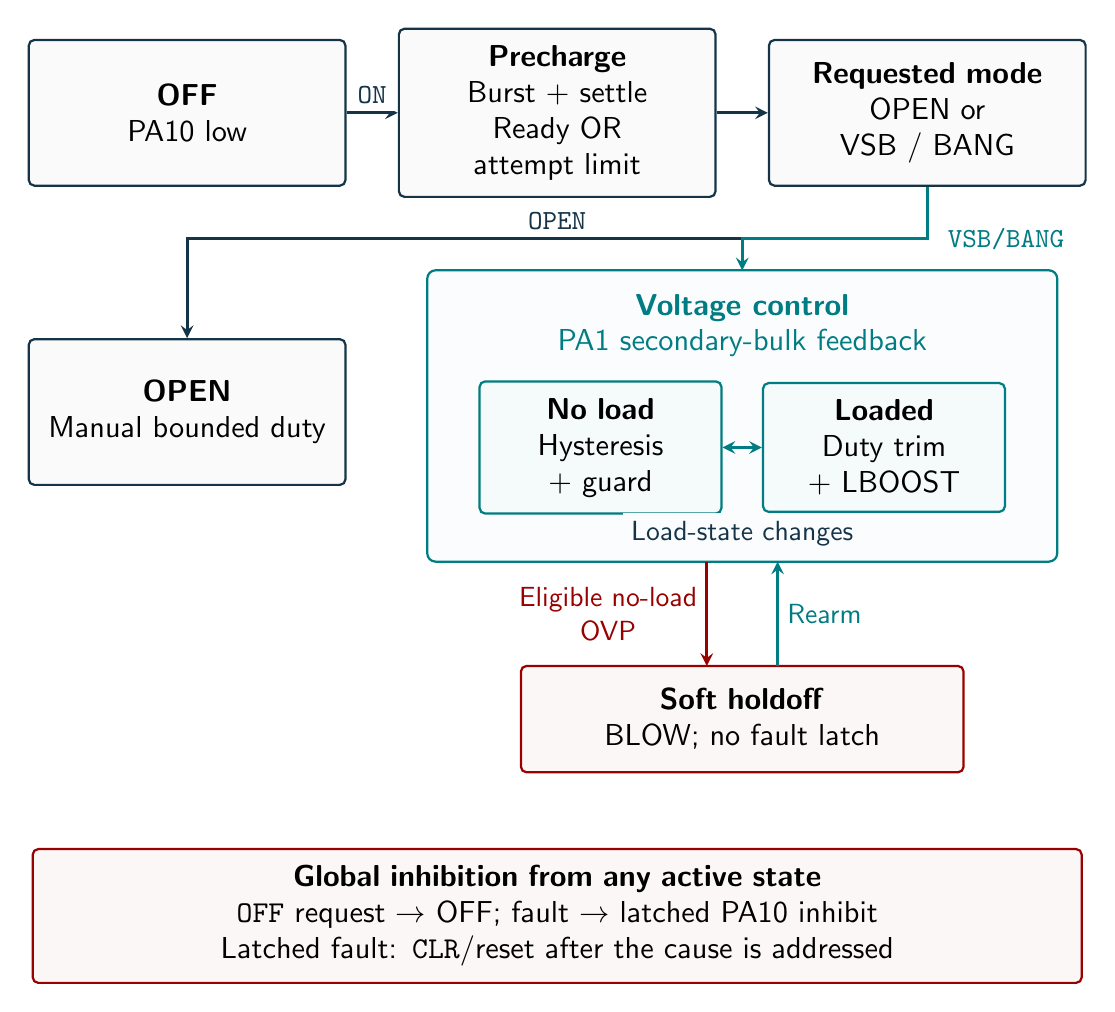
\begin{tikzpicture}[
font=\sffamily\fontsize{11}{13}\selectfont,
every node/.style={align=center,inner sep=6pt,
    execute at begin node={\hyphenpenalty=10000\exhyphenpenalty=10000}},
state/.style={draw=ctrlnavy,fill=black!2,rounded corners=2pt,
    line width=0.8pt,text width=3.6cm,minimum height=1.85cm},
run/.style={state,draw=ctrlteal,fill=ctrlteal!4},
hold/.style={state,draw=ctrlred,fill=ctrlred!3,minimum height=1.35cm},
flow/.style={->,>=stealth,draw=ctrlnavy,line width=1.0pt},
runflow/.style={flow,draw=ctrlteal},
inhibit/.style={flow,draw=ctrlred},
annotation/.style={font=\sffamily\fontsize{10}{12}\selectfont,text=ctrlnavy,
    inner sep=3pt,fill=white}]
\node[state] (off) at (0,0) {\textbf{OFF}\\PA10 low};
\node[state] (pre) at (4.7,0)
    {\textbf{Precharge}\\Burst + settle\\Ready OR attempt limit};
\node[state] (mode) at (9.4,0)
    {\textbf{Requested mode}\\OPEN or\\VSB / BANG};
\node[state] (open) at (0,-3.8)
    {\textbf{OPEN}\\Manual bounded duty};
\draw[draw=ctrlteal,fill=ctrlteal!2,rounded corners=3pt,line width=0.8pt]
    (3.05,-2.0) rectangle (11.05,-5.7);
\node[text=ctrlteal] at (7.05,-2.7)
    {\textbf{Voltage control}\\PA1 secondary-bulk feedback};
\node[run,text width=2.65cm,minimum height=1.4cm] (light) at (5.25,-4.25)
    {\textbf{No load}\\Hysteresis + guard};
\node[run,text width=2.65cm,minimum height=1.4cm] (loaded) at (8.85,-4.25)
    {\textbf{Loaded}\\Duty trim + LBOOST};
\node[annotation,fill=ctrlteal!2] at (7.05,-5.35) {Load-state changes};
\node[hold,text width=5.2cm] (soft) at (7.05,-7.7)
    {\textbf{Soft holdoff}\\BLOW; no fault latch};
\node[hold,text width=12.9cm,minimum height=1.6cm] at (4.7,-10.2)
    {\textbf{Global inhibition from any active state}\\
    \texttt{OFF} request $\rightarrow$ OFF; fault $\rightarrow$ latched PA10 inhibit\\
    Latched fault: \texttt{CLR}/reset after the cause is addressed};
\draw[flow] (off) -- node[annotation,above] {\texttt{ON}} (pre);
\draw[flow] (pre) -- (mode);
\draw[flow] (mode.south) -- (9.4,-1.6) --
    node[annotation,above] {\texttt{OPEN}} (0,-1.6) -- (open.north);
\draw[runflow] (mode.south) -- (9.4,-1.6) -- (7.05,-1.6) -- (7.05,-2.0);
\node[annotation,text=ctrlteal,anchor=west] at (9.55,-1.6) {\texttt{VSB/BANG}};
\draw[runflow,<->] (light) -- (loaded);
\draw[inhibit] (6.6,-5.7) -- node[annotation,left,text=ctrlred]
    {Eligible no-load\\OVP} (6.6,-7.025);
\draw[runflow] (7.5,-7.025) -- node[annotation,right,text=ctrlteal]
    {Rearm} (7.5,-5.7);
\end{tikzpicture}
\endgroup
\caption{Baseline firmware states. OPEN selects manual duty; voltage control switches between loaded and no-load operation and can enter soft holdoff at \texttt{BLOW} (default zero). OFF and latched faults force PA10 low.}
\label{fig:ctrl-state-diagram}
\end{figure}

\begin{table}[htbp]
\centering
\caption{Firmware states, actions, and exit conditions.}
\label{tab:ctrl-state-machine}
\begin{tabularx}{\textwidth}{@{}p{0.22\textwidth}Xp{0.29\textwidth}@{}}
\toprule
State & Action & Exit condition\\
\midrule
OFF & Configure peripherals and hold PA10 low & Valid \texttt{ON} request\\
Precharge & Alternate small energy packets and settling & Readiness threshold or attempt limit, OFF, or fault\\
OPEN & Apply the operator's bounded enable command & Mode change, OFF, or fault\\
Voltage control & Use PA1 thresholds with loaded/no-load behavior & Mode change, OFF, or fault\\
Soft holdoff & Request \texttt{BLOW} (default zero) without latching & Voltage reaches rearm condition, OFF, or fault\\
Fault latched & Inhibit PA10 & \texttt{CLR} or reset after the cause is addressed\\
\bottomrule
\end{tabularx}
\end{table}

Startup proceeds when \texttt{PREV} is reached \emph{or} \texttt{PREMAX} is exhausted. Exhausting attempts does not itself latch a dedicated startup fault. Other fault checks remain active. A timed startup trace must therefore include feedback voltage and state to show why normal operation began.

\texttt{OPEN} selects manual duty; \texttt{VSB}/\texttt{BANG} selects voltage control. Runtime enable is separate from \texttt{BOOTON}/\texttt{BOOTOFF}, which save the boot preference. \texttt{OFF} inhibits transfer. Any charge in the link and output capacitors remains until discharged through the available paths.

\section{Fault Detection and Recovery}
\label{sec:ctrl-faults}

The baseline checks the ADC/DMA acquisition-running flag and optional PA2 current trip before voltage control. A cleared running flag latches \texttt{SENSOR}; the flag alone does not detect every conversion or transfer error. With current trip enabled, a primary-current reading above threshold latches \texttt{CURRENT}. Both faults force burst enable at PA10 low on the original prototype. Current trip is disabled by default, and the active voltage loop does not call the legacy current-foldback helper even with \texttt{IFOLDEN} enabled.

With \texttt{OVPEN} enabled, a filtered or latest raw secondary-voltage reading from PA1 above \texttt{OVP} normally latches an \texttt{OVP} fault. Eligible light/no-load operation has a recoverable exception when soft protection is enabled. The low-duty request can be held without latching only while every relevant voltage estimate stays at or below
\begin{equation}
 V_{\mathrm{hard,NL}}=
 \min\!\left(V_{\mathrm{OVP}}+\SI{4}{\volt},\SI{80}{\volt}\right).
 \label{eq:ctrl-no-load-hard-limit}
\end{equation}
Above that ceiling, or outside the eligibility conditions, the normal hard check applies. With the default \SI{36}{\volt} OVP value, the eligible exception extends to \SI{40}{\volt}. This higher threshold must be included when checking voltage stress.

The normal soft holdoff is triggered at \texttt{NLSOVP} and rearms below \texttt{NLSOVPR}, defaulting to \SI{33.5}{\volt} and \SI{23}{\volt}. The configured low duty is requested, allowing no-load operation to recover without an operator reset. The response still depends on current classification and voltage conversion.

A latched fault must be cleared with \texttt{CLR} or reset before transfer resumes. The status name \texttt{MAX\_DUTY} remains from the earlier power-control work, but the final voltage path does not call that protection function. It cannot serve as an active output-power limit.

These checks use the same MCU, sensing, and actuator as regulation. Trigger, enable inhibition, and recovery must be captured together in the next protection test. There is no separate hardware protection channel in these firmware checks.

\section{Control Timing and Settings}
\label{sec:ctrl-timing}

The default \texttt{CPER} of \SI{25}{\micro\second} requests \SI{40}{\kilo\hertz} foreground updates. UART presets also provide \SI{20}{\micro\second}, \SI{50}{\micro\second}, and \SI{100}{\micro\second}. Elapsed-time scheduling allows interrupts and foreground work to extend the actual interval.

\texttt{STATUS} was used to inspect the last and maximum control intervals, overruns, ADC snapshot time, DMA state, requested and effective duty, envelope timing, skipped periods, and carrier-sync counts. These software fields help locate delays; an external capture is needed to measure the jitter distribution and its relationship to the switching waveform.

Firmware version, calibration, thresholds, loaded/no-load settings, and timing affect the control response and should be recorded with each test. Appendix~\ref{app:firmware} gives the command reference.

\section{V2 Controller Port and Browser Interface}
\label{sec:ctrl-pwr2-port}

The V2 port replaces the STM32G071 Nucleo arrangement with an integrated STM32F410CBU6. Conditional definitions retain support for both MCU targets while adapting the complementary carrier, enable timer, ADC/DMA configuration, and settings storage. The baseline voltage-control law was retained. Browser control and UART logging were followed by automatic calibration, editable reference-load settings, and adjustable carrier timing. The earlier DMA feedback development is described in Section~\ref{sec:ctrl-v2}.

Commands and functions are listed in Appendix~\ref{app:firmware}.

\subsection{Peripheral Changes}

On V2, the complementary carrier uses PA8/TIM1\_CH1 and PB13/TIM1\_CH1N, with burst enable moved to PA11. This releases PA9/PA10 for UART TX/RX; PA10 therefore changes from G071 burst enable to F410 serial receive. The complementary outputs share the TIM1 compare signal and hardware dead-time generator \cite{ststm32f410ds,ststm32f410rm}. The earlier port used center-aligned counting; the adjustable implementation uses edge-aligned counting with equal reference pulse widths. The default remains a \SI{1}{\mega\hertz} carrier with \SI{40}{\nano\second} programmed dead time.

\begin{table}[htbp]
\centering
\caption{MCU pin and peripheral changes from the baseline controller to V2.}
\label{tab:ctrl-pwr2-port}
\small
\begin{tabularx}{\textwidth}{@{}L{0.23\textwidth}L{0.31\textwidth}Y@{}}
\toprule
Function & STM32G071 baseline & STM32F410 V2 target\\
\midrule
Carrier & PA8/PA9; TIM1 CH1/CH2 & PA8/PB13; TIM1 CH1/CH1N\\
Burst enable & PA10; TIM3 scheduler & PA11; TIM5 scheduler\\
UART & PC5 RX, PC4 TX & PA10 RX, PA9 TX; USART1\\
Feedback & PA0, PA1, PA2; ADC1 & Same feedback inputs on the same MCU pins\\
ADC transfer & DMA1 Channel 1 & DMA2 Stream 0, Channel 0\\
Saved settings & Four EEPROM-emulation slots & Reserved 16 KiB flash journal\\
\bottomrule
\end{tabularx}
\end{table}

The free-running ADC scan samples primary voltage, secondary-bulk voltage, and primary current sequentially, without synchronization to the carrier. At the selected \SI{25}{\mega\hertz} clock, 84 sampling plus 12 conversion cycles give \SI{3.84}{\micro\second} per channel and \SI{11.52}{\micro\second} per scan, about 86.8 thousand scans per second. ADC overrun and DMA errors are polled during filter updates to route detected acquisition failures to the sensor-fault path.

The port retains the earlier conversion defaults. The repeated \SI{6.2}{\mega\ohm} schematic labels need checking against the fitted resistors. The voltage, current, and protection scales must use the measured circuit gains.

\subsection{Saving MCU Settings}

The V2 MCU has no dedicated EEPROM. Sector 1 at \texttt{0x08004000} was reserved for settings. Application code was placed at \texttt{0x08008000}, with vectors at the normal flash base. The linker script and startup layout check keep program data outside the settings sector.

Each save appends a sequence-numbered, checksummed entry and verifies it by reading it back. Occupied entries are skipped after interrupted programming, and successive saves use different entries across the sector. When the journal wraps, the sector is erased; an interruption during erase can remove the saved configuration. If no valid entry remains, defaults load with output OFF. Writes wait until output, startup, and autotuning are inactive so flash work does not interrupt live conversion.

Timing and calibration are saved together in a 488-byte record, giving 33 entries in the reserved sector. Existing settings from the earlier format load with default carrier timing and are not rewritten at startup. Older firmware cannot read the new record format.

The saved boot preference was kept separate from runtime \texttt{ON}/\texttt{OFF}. To keep calibration during a firmware update, the programming method must preserve the settings sector. OFF inhibits transfer; it does not remove charge already stored in the converter.

\subsection{Browser Commands Without Blocking Control}

An opt-in browser protocol was added to the V2 firmware over the existing \SI{115200}{baud} UART. \texttt{WEB HELLO} selects JSON replies without enabling output. Command IDs and acknowledgments show whether the MCU accepted a change. On the MCU, input is limited to 96 characters, the transmit queue has four fixed-size frames, and each loop pass sends at most 16 bytes when the UART has space. Periodic samples are dropped when the queue is congested so old telemetry does not delay the controller.

Browser \texttt{ON} also requires an active communication lease. The host renews it with \texttt{PING}. Expiry requests enable inhibition before an event is formatted. This check runs in the background loop and depends on execution continuing. Calibration routines service UART commands and cancellation checks during their waits, allowing OFF and lease expiry to interrupt a run. A browser settings save requires OFF. Pending RAM changes and completed flash saves are reported separately.

The browser reports \texttt{vsec} as bulk voltage before the MPQ4242, \texttt{current} as the primary half-bridge-current estimate derived from input PA2, and \texttt{power} as their selected diagnostic voltage--current product. External output measurements are still needed for performance calculations. Displayed duty comes from scheduler state and needs a scope check when assessing actual enable timing.

\subsection{Automatic Calibration and Reference Loads}

Browser calibration was added for startup precharge, no-load operation, and three reference loads. For no-load and reference-load tuning, the existing coarse and fine search is used to find a burst duty from the measured secondary-bulk voltage. The burst-enable frequency remains fixed during this search. This makes the earlier terminal routines accessible from the setup interface without adding a separate control algorithm.

Each reference load is connected by the operator, and its resistance is entered in the setup page. The resistance entry describes the connected load; it does not set an electronic load or switch a resistor. Selecting a calibrated slot applies its stored profile. No-load duty, scan step and interval, and startup precharge settings can also be read and adjusted with output OFF. Current-zero capture corrects the current-sense offset. Primary-voltage-reference capture sets the line-feed-forward reference.

A calibration run starts with output OFF and leaves it OFF after completion. OFF, communication-lease expiry, a fault, or the \SI{180}{\second} timeout cancels the run; interrupted or failed runs restore the previous settings. Successful browser changes remain in RAM until explicitly saved with the output disabled.

\subsection{Adjustable Carrier Frequency and Dead Time}
\label{sec:ctrl-v2-adjustable-timing}

Carrier frequency and dead time were made adjustable so that switching could be set relative to the modified resonant tank and the commutation interval could be varied without rebuilding the firmware. Both values are applied together through \texttt{TIMING} while output is OFF and startup and calibration are inactive. Burst duty continues to regulate the secondary bulk voltage. The separate \texttt{FEN} setting controls the burst-enable frequency; the tank's natural resonant frequency is set by its inductance and capacitance.

The command accepts carrier requests from \SI{500}{\kilo\hertz} to \SI{2}{\mega\hertz} and dead-time requests from \SI{20}{\nano\second} to \SI{200}{\nano\second}. These are timer-setting limits. The converter operating range still needs switching and thermal measurements. TIM1 uses an even period count for balanced reference pulses, and dead time is rounded up to a timer count. At a \SI{100}{\mega\hertz} timer clock, period increments are \SI{20}{\nano\second} and dead-time increments are \SI{10}{\nano\second}. Frequency steps therefore depend on the selected period.

For timer clock \(f_t\), period count \(N_p\), and dead-time count \(N_d\), the applied settings are
\begin{equation}
 f_s=\frac{f_t}{N_p},\qquad t_d=\frac{N_d}{f_t},\qquad 4N_d<N_p.
 \label{eq:ctrl-v2-carrier-timing}
\end{equation}
The last condition rejects pairs that leave insufficient pulse time. A request of \SI{950}{\kilo\hertz} and \SI{53}{\nano\second}, for example, gives \(N_p=106\) and \(N_d=6\): approximately \SI{943.396}{\kilo\hertz} and \SI{60}{\nano\second}. The browser displays the applied values from MCU readback, and burst scheduling uses the actual clock and period counts.

Changing either applied timer count clears the three learned load profiles and tuning results. Reference resistances, sensor calibration, and applied duty settings are retained. Calibration must then be repeated before using learned profiles at the new timing. Browser timing changes require an explicit save while OFF; the terminal retains its existing automatic save after a \SI{1.5}{\second} quiet interval while OFF, unless a configuration import is active.

The programmed interval is the separation between timer output commands. Driver delay and switch-node commutation determine the effective transistor dead time, which must be measured on the assembled board. The duty-search calibration holds carrier frequency fixed.

\subsection{Software Verification}

The V2 firmware, protocol tests, settings-storage tests, and browser tests were built and checked. These checks cover timer rounding and pair rejection, application with output disabled, learned-profile clearing, calibration cancellation, and saved-settings recovery after interrupted writes.

Powered validation of the adjustable implementation remains to be completed. The V1.0 measurements and later V2 thermal observations in Chapter~\ref{ch:results} describe the earlier test configurations. Switching waveforms and matched electrical and thermal measurements are needed to assess the new timing controls on the converter.



